\documentclass[12pt]{article}

\usepackage[brazilian]{babel}
\usepackage[utf8]{inputenc}
\usepackage{graphicx}
\usepackage{mathtools}
\usepackage{amsthm}
\usepackage{thmtools,thm-restate}
\usepackage{amsfonts}
\usepackage{hyperref}
\usepackage[singlelinecheck=false]{caption}
\usepackage[backend=biber,url=true,doi=true,eprint=false,style=numeric]{biblatex}
\usepackage{enumitem}
\usepackage[justification=centering]{caption}
\usepackage{indentfirst}
\usepackage{algorithm}
\usepackage{algpseudocode}
\usepackage{listings}
\usepackage[x11names,rgb,table]{xcolor}
\usepackage{tikz}
\usepackage{hyperref}
\usepackage{subcaption}
\usepackage{booktabs}
\usepackage{linegoal}
\usepackage{geometry}
\usetikzlibrary{snakes,arrows,shapes}

\addbibresource{references.bib}
\graphicspath{{imgs/}}

\makeatletter
\def\subsection{\@startsection{subsection}{3}%
  \z@{.5\linespacing\@plus.7\linespacing}{.1\linespacing}%
  {\normalfont}}
\makeatother

\makeatletter
\patchcmd{\@setauthors}{\MakeUppercase}{}{}{}
\makeatother

\DeclareMathOperator*{\argmin}{arg\,min}
\DeclareMathOperator*{\argmax}{arg\,max}
\DeclareMathOperator*{\Val}{\text{Val}}
\DeclareMathOperator*{\Ch}{\text{Ch}}
\DeclareMathOperator*{\Pa}{\text{Pa}}
\DeclareMathOperator*{\Sc}{\text{Sc}}
\newcommand{\ov}{\overline}
\newcommand{\tsup}{\textsuperscript}

\newcommand\defeq{\mathrel{\overset{\makebox[0pt]{\mbox{\normalfont\tiny\sffamily def}}}{=}}}

\newcommand{\algorithmautorefname}{Algorithm}
\algrenewcommand\algorithmicrequire{\textbf{Input}}
\algrenewcommand\algorithmicensure{\textbf{Output}}
\algnewcommand{\LineComment}[1]{\State\,\(\triangleright\) #1}

\captionsetup[table]{labelsep=space}

\theoremstyle{plain}

\newcounter{dummy-def}\numberwithin{dummy-def}{section}
\newtheorem{definition}[dummy-def]{Definition}
\newcounter{dummy-thm}\numberwithin{dummy-thm}{section}
\newtheorem{theorem}[dummy-thm]{Theorem}
\newcounter{dummy-prop}\numberwithin{dummy-prop}{section}
\newtheorem{proposition}[dummy-prop]{Proposition}
\newcounter{dummy-corollary}\numberwithin{dummy-corollary}{section}
\newtheorem{corollary}[dummy-corollary]{Corollary}
\newcounter{dummy-lemma}\numberwithin{dummy-lemma}{section}
\newtheorem{lemma}[dummy-lemma]{Lemma}
\newcounter{dummy-ex}\numberwithin{dummy-ex}{section}
\newtheorem{exercise}[dummy-ex]{Exercise}
\newcounter{dummy-eg}\numberwithin{dummy-eg}{section}
\newtheorem{example}[dummy-eg]{Example}

\numberwithin{equation}{section}

\newcommand{\set}[1]{\mathbf{#1}}
\newcommand{\pr}{\mathbb{P}}
\newcommand{\eps}{\varepsilon}
\newcommand{\ddspn}[2]{\frac{\partial#1}{\partial#2}}
\newcommand{\iddspn}[2]{\partial#1/\partial#2}
\renewcommand{\implies}{\Rightarrow}

\newcommand{\bigo}{\mathcal{O}}

\setlength{\parskip}{1em}

\lstset{frameround=fttt,
	numbers=left,
	breaklines=true,
	keywordstyle=\bfseries,
	basicstyle=\ttfamily,
}

\newcommand{\code}[1]{\lstinline[mathescape=true]{#1}}
\newcommand{\mcode}[1]{\lstinline[mathescape]!#1!}

\newgeometry{margin=1in}
\title{%
  \vspace{-3.0cm}
  {
\includegraphics[scale=0.2]{logo-usp.png}}\\
  {\textbf{\uppercase{\Large USP --- Universidade de São Paulo}}}\\
  \vspace{1.5cm}
  {\textbf{Aprendizagem automática de redes soma-produto}}\\
  \vspace{2.0cm}
\flushleft{\Large Relatório Parcial de Projeto de Iniciação Científica\\
PIBIC Projeto 800585/2016\texttt{-}0}\\
  \vspace{2.5cm}
\flushleft{\Large Bolsista: Renato Lui Geh\\
Orientador: Prof.\ Dr.\ Denis Deratani Mauá}\\
  \vspace{2.5cm}
  \centering
  {\Large\textbf{São Paulo}}\\
  \vspace{0.25cm}
  {\Large\textbf{2018}}\\
}
\date{}

\begin{document}

\maketitle

\section{Introdução}

Este relatório parcial descreve as atividades realizadas no projeto PIBIC 800585/2016\texttt{-}0
durante o período de 01/08/2017 e 31/01/2018. Nesta seção, serão enunciados os objetivos do
projeto. Em seguida, as atividades desenvolvidas durante o período serão descritas. Também serão
explicados os problemas encontrados durante o projeto. Em fim, serão mostrados resultados
parciais do projeto e apresentando uma breve conclusão do trabalho parcial do projeto.

Modelos probabilísticos baseados em grafos (PGM, do inglês \textit{Probabilistic Graphical Models})
representam uma distribuição de probabilidade de forma compacta. Estes modelos representados por
grafos facilitam tanto a compreensão humana ao estudá-los, quanto possibilitam que vários problemas
já existentes em Teoria dos Grafos sejam utilizados como solução para problemas em PGMs. Extrair
conhecimento de PGMs é análogo a extrair a probabilidade de um certo evento ocorrer dado que
eventos distintos tenham ocorrido. Tal extração de conhecimento é chamada de inferência. Fazer
inferência exata em PGMs clássicas, ou seja, acharmos a probabilidade exata de um certo evento, é
intratável. Uma solução para este problema é utilizarmos métodos para inferência aproximada nestes
modelos. No entanto, tais algoritmos aproximados são muitas vezes difíceis de analisar. Além disso,
como os algoritmos de aprendizado do modelo utilizam inferência como subrotina, por consequência o
aprendizado torna-se aproximado.

\begin{figure}[h]
  \centering
  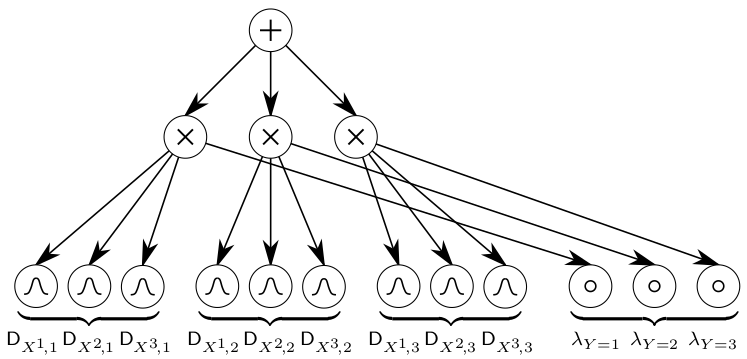
\includegraphics[scale=0.4]{nbayes.png}
  \caption{}\label{spn-example}
\end{figure}

Redes soma-produto (SPN, de \textit{Sum-Product Network}) são PGMs que representam uma distribuição
de probabilidade tratável. Proposto em 2011, SPNs computam inferência exata em tempo linear ao
número de arestas de seu grafo se sua estrutura obedecer a certas
propriedades~\cite{poon-domingos}. A~\autoref{spn-example} mostra um exemplo de rede soma-produto
representando o modelo Naïve Bayes com três atributos. SPNs apresentam uma série de características
interessantes, como sua arquitetura profunda que permite representar funções de forma mais
eficiente quanto mais profundo seu grafo~\cite{shallow-vs-deep}. Outras interessantes propriedades
teóricas incluem uma generalização de SPNs para qualquer semianel em que o produto tenha escopo
disjunto~\cite{sp-theorem}. Com relação a aplicações, SPNs tiveram resultados impressionantes em
diversas áreas, como enovelamento de proteínas~\cite{rec-dec-non-convex}, modelagem de
sinais~\cite{model-speech}, classificação e reconstrução de
imagens~\cite{gens-domingos,poon-domingos,clustering}, reconhecimento de atividade~\cite{activity}
e linguagem natural~\cite{nat-lang}.

Neste projeto, pretende-se desenvolver uma biblioteca livre e gratuita para inferência e algoritmos
de aprendizado estado-da-arte em SPNs, analisando-se experimentalmente tais algoritmos em tarefas
reais, como compleição e classificação de imagens.

\section{Cronograma e acompanhamento}

O cronograma original planejado para o projeto PIBIC é descrito abaixo, com o símbolo \checkmark{}
usado para representar as atividades concluídas e $\times$ para atividades não terminadas.

\begin{table}[h]
  \centering
  \begin{tabular}{|c|c|c|c|c|c|c|}
    \hline
    Atividade/Mês & 1\tsup{o}--2\tsup{o} & 3\tsup{o}--4\tsup{o} & 5\tsup{o}--6\tsup{o} &
    7\tsup{o}--8\tsup{o} & 9\tsup{o}--10\tsup{o} & 11\tsup{o}--12\tsup{o} \\ \hline
    a & \checkmark{} & & & & & \\ \hline
    b & \checkmark{} & & & & & \\ \hline
    c & & \checkmark{} & & & & \\ \hline
    d & & $\times$ & & & & \\ \hline
    e & & & \checkmark{} & & & \\ \hline
    f & & & & $\times$ & & \\ \hline
    g & $\times$ & $\times$ & \checkmark{} & $\times$ & & \\ \hline
    h & & & & & $\times$ & \\ \hline
    i & & & & & $\times$ & $\times$ \\ \hline
    j & & & & & & $\times$ \\ \hline
  \end{tabular}
\end{table}

\begin{enumerate}[label=\alph*.]
  \item Estudo de conceitos de SPN\@.
  \item\label{lbl-c-pd} Estudo e implementação do algoritmo de aprendizado de Poon e Domingos
    (2011)~\cite{poon-domingos}.
  \item\label{lbl-c-ds} Estudo e replicação da rede para compleção de imagens descrita em Poon e
    Domingos (2011).
  \item\label{lbl-c-vd} Estudo e implementação do algoritmo de aprendizado de estrutura de Ventura
    e Dennis (2012)~\cite{clustering}.
  \item Estudo e implementação do algoritmo de aprendizado de estrutura de Gens e Domingos
    (2013)~\cite{gens-domingos}.
  \item\label{lbl-c-vm} Estudo e implementação do algoritmo de aprendizado de estrutura de Vergari
    e di Mauro (2016)~\cite{vergari-mauro}.
  \item Avaliação de desempenho de algoritmos em problemas de compleição de imagem.
  \item Elaboração de artigo para ENIAC 2018.
  \item Relatório e participação no SIICUSP\@.
  \item Disponibilização da biblioteca e documentação do código.
\end{enumerate}

Os itens~\ref{lbl-c-pd} e~\ref{lbl-c-ds}, assim como a avaliação do desempenho vinculado ao
algoritmo, geraram vários problemas com relação a implementação, causando atraso no cronograma.
Esses problemas são detalhados na~\autoref{sct-prob}. Apesar do atraso, planeja-se manter o
cronograma atual, realizando-se as atividades descritas nos itens~\ref{lbl-c-vd} e~\ref{lbl-c-vm}
durante os subsequentes meses.

\section{Atividades desenvolvidas}

O objetivo do projeto é o desenvolvimento de uma biblioteca livre e gratuita para inferência e
aprendizado de SPNs. O nome dado a biblioteca foi GoSPN e encontra-se disponível em
\url{https://github.com/RenatoGeh/gospn}. A linguagem de programação escolhida foi Go. Essa escolha
deu-se por causa de sua sintaxe simples, tempo de compilação e execução rápidos, e suporte nativo
para programação concorrente e paralela. Foram implementadas diversas funcionalidades à biblioteca,
que serão enumeradas a seguir e em seguida exploradas em mais detalhes.

\begin{enumerate}
  \item Inferência por marginais e MAP;\label{lbl-inference}
  \item Derivadas em função da rede e pesos;\label{lbl-derivative}
  \item Aprendizado generativo por descida de gradiente;\label{lbl-generativegd}
  \item Aprendizado estrutural de Gens-Domingos;\label{lbl-gensdomingos}
  \item Geração de estrutura densa (Poon-Domingos);\label{lbl-dense}
  \item Suporte para conjuntos de dados ARFF para variáveis discretas;\label{lbl-arff}
  \item Testes de completude e decomponibilidade.\label{lbl-cc}
\end{enumerate}

Os itens~\ref{lbl-inference},~\ref{lbl-gensdomingos} e~\ref{lbl-arff} foram implementados antes do
início da bolsa.

Redes soma-produto são DAGs cujos nós podem ser nós somas, em que o valor da soma é a média
ponderada de seus filhos; nós produtos, cujos valores são o produtório de seus filhos; ou folhas,
que representam distribuições de probabilidade univariadas. O valor de uma SPN é o valor de sua
raíz. O escopo de um nó da SPN é a união entre o escopo de seus filhos. O escopo de uma folha é o
escopo da distribuição de probabilidade.

Computar inferência por marginais equivale a achar a probabilidade de um evento dada uma evidência.
Em redes soma-produto, computar tal probabilidade consiste em achar o valor da raíz da SPN dados
valores pré-determinados de certas variáveis. Foram implementadas duas funções na biblioteca para
computar os marginais. A primeira é um método de classe que utiliza recorrência para achar o valor
dos subsequentes filhos de forma \textit{top-down}. A segunda é uma função estática que usa
programação dinâmica para evitar recomputar valores. Adicionalmente, esta função usa uma estrutura
de dados para armazenar os nós visitados, evitando usar a pilha de chamada.

A probabilidade maximum-a-posteriori (MAP) é uma estimativa do evento mais provável de se ocorrer
dada uma evidência. De forma análoga a computar os marginais, GoSPN permite usar duas funções para
computar o MAP\@. Computar o MAP em SPNs é NP-difícil~\cite{peharz-spn,cmc2017}. Em GoSPN,
implementamos um algoritmo aproximado apresentado por~\cite{poon-domingos}.

Aprendizado generativo por descida de gradiente em redes soma-produto é realizado computando as
derivadas da rede em função dos seus parâmetros. GoSPN possue várias funções para achar as
derivadas dadas instâncias. Também foram implementadas versões para computar as derivadas em lote.
Após achadas as derivadas, é possível atualizar os parâmetros da rede aplicando o gradiente. Em
GoSPN, foi implementado apenas o aprendizado de parâmetros por descida de gradiente de forma
generativa.

Diz-se aprendizado de parâmetros quando atualizam-se apenas os pesos da SPN\@. O aprendizado
estrutural de SPNs ajusta tanto os pesos quanto o grafo da rede. Foi criada uma implementação do
esquema de algoritmo de aprendizado estrutural de Gens e Domingos. Em~\cite{gens-domingos}, é dada
certa liberdade quanto a certos pontos do algoritmo. O esquema é composto por três casos executados
recursivamente:

\begin{algorithm}[H]
  \caption*{\code{LearnSPN}~\cite{gens-domingos}}
  \begin{algorithmic}[1]
    \Require\,Dataset $\mathbf{D}=(I,X)$, onde $I$ é o conjunto de instâncias e $X$ o conjunto de
    variáveis
    \Ensure\,SPN representando a distribuição de probabilidade de $I$ sobre as variáveis $X$
    \If{$|X|=1$}
      \State\,\textbf{return} distribuição de probabilidade univariada de $I$
    \Else%
      \State\,Particione $X$ em $P_1,P_2,\ldots,P_m$ tal que todo $P_i$ é independente de $P_j$,
      $i\neq j$
      \If{$m>1$}
        \State\,\textbf{return} nó produto cujos filhos são as recorrências
        \mcode{LearnSPN$(I,P_i)$}, para todo $1\leq i\leq m$
      \Else%
        \State\,Rode \textit{clustering} em $I$ tal que $Q_1,Q_2,\ldots,Q_n$ são os clusters de $I$
        \State\,\textbf{return} nó soma cujos filhos são as recorrências \mcode{LearnSPN$(Q_i,X)$}
        com peso $|Q_i|/|I|$
      \EndIf%
    \EndIf%
  \end{algorithmic}
\end{algorithm}

Em GoSPN, foram implementados os algoritmos de \textit{clustering} DBSCAN e $k$-\textit{means}.
Para os testes de independência foram implementados o teste de $\chi^2$ e \textit{G-test}.

Para replicação dos resultados obtidos em~\cite{poon-domingos}, assim como validação dos algoritmos
de aprendizado de parâmetros, fez-se necessária a implementação da estrutura densa descrita
em~\cite{poon-domingos}. O algoritmo de geração de tal estrutura cria uma rede adequada para
conjuntos de dados que apresentam dependência local entre variáveis. Este tipo de estrutura é
aplicável a compleição e classificação de imagens, já que \textit{pixels} vizinhos apresentam
coloração semelhante. A geração desta estrutura depende principalmente de três parâmetros, o número
de nós somas por cada região retangular da imagem, denotada por $m$; o número de distribuições
gaussianas por pixel, denotada por $g$; e o menor nível de resolução da imagem em pixels, $r$.

Para validação dos algoritmos, é interessante utilizar conjuntos de dados de diferentes aplicações
do mundo real. Para tanto, foi necessário adotar um formato padronizado. Foi implementado suporte
para o formato ARFF, que é extensamente usado pela comunidade.

Além da validação empírica, também é importante verificar propriedades da rede. Uma SPN é completa
quando todo nó soma tem mesmo escopo que seus filhos, e é consistente quando nenhuma variável tem
valorações distintas nos filhos de um mesmo nó produto. Quando uma SPN é completa e consistente
diz-se que ela é válida. Uma SPN válida computa a probabilidade exata de uma evidência. A SPN $S$ é
decomponível se, em um nó produto de $S$, os escopos dos filhos são disjuntos. Decomponibilidade
implica em consistência, além do que SPNs consistentes não são mais compactas que SPNs
decomponíveis~\cite{theoretical-spn}. Foram implementadas funções que verificam se uma SPN é
completa ou decomponível.

Além de funções que tem relação direta com redes soma-produto, também foi necessário implementar
algoritmos clássicos de teoria dos grafos. Foram criadas funções para busca-em-profundidade,
busca-em-largura, achar uma \textit{spanning tree} de um grafo, e encontrar a ordem topológica de
um DAG\@.

\section{Problemas encontrados}\label{sct-prob}

Em~\cite{poon-domingos}, os autores não explicam de forma explícita as etapas para o algoritmo de
aprendizado por descida de gradiente. Adicionalmente não foram encontradas implementações do
algoritmo de aprendizado generativo por descida de gradiente. O artigo de Poon e Domingos comenta
que aprendizado por descida de gradiente se dá naturalmente por
\textit{backpropagation}\cite{poon-domingos}, no entanto o código anexado não apresenta nenhuma
implementação do algoritmo. Além disso, uma busca por implementações disponíveis indica a falta
de uma implementação generativa por descida de gradiente. Por tanto, foram feitas certas suposições
com relação à implementação. Foram utilizados comentários sobre o algoritmo contidos nos
artigos~\cite{poon-domingos,discriminative} para tal implementação.

O tamanho da rede gerada pelo algoritmo de estrutura densa de Poon e Domingos também mostrou-se
problemática. O número de nós no grafo gerado com uma imagem $46\times 56$ e com parâmetros $m=4$,
$g=4$ e $r=4$ foi 1.701.333. O tempo total gasto no aprendizado de tal SPN foi de aproximadamente 6
horas e ocupou 1GB de memória. No entanto, tais parâmetros usados são considerados pequenos, já que
os parâmetros usados no artigo original foram $m=20$, $g=4$ e $r=4$ em uma imagem de tamanho
$64\times 64$. Ao gerarmos o grafo com tais parâmetros, excedeu-se a memória de 16GB\@. No artigo
original, foi usado um \textit{cluster} de 48 máquinas com 8 processadores e 16GB de memória cada,
o que explica a discrepância.

Ao final da implementação do algoritmo de Poon e Domingos, os resultados extraídos a partir dos
conjuntos de dados escolhidos mostraram-se incompatíveis com o esperado. Para resolver tal
problema, planeja-se fazer diversos testes nas implementações da estrutura e algoritmo de
aprendizado de Poon e Domingos.

\section{Resultados}

Até o momento foi apenas possível extrair resultados do algoritmo de aprendizado estrutural de Gens
e Domingos. Tanto a implementação como a extração dos resultados foram realizadas antes do início
da bolsa. Foram utilizados três conjuntos de dados: Caltech-101~\cite{caltech101}, Olivetti Faces e
Digits.

O primeiro contém imagens de diferentes dimensões e resoluções de 101 categorias de
objetos. Foram escolhidas as categorias carro, motos e faces. As imagens foram padronizadas e
redimensionadas em imagens em escala de cinza com 150 de largura e 65 de altura em resolução de
8-bits. O \textit{dataset} está disponível em
\url{http://www.vision.caltech.edu/Image_Datasets/Caltech101/}.

\begin{figure}[h]
  \centering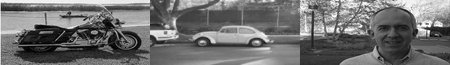
\includegraphics[scale=1.0]{imgs/caltech_sample.png}
  \caption{Uma amostra do conjunto de dados Caltech-101.}
\end{figure}

O segundo é um conjunto de imagens de faces, com diferentes expressões e ângulos. As imagens têm
dimensões $46\times 56$ com resolução de 8-bits em escala de cinza. Como a distribuição de cores é
irregular, com nenhum pixel tendo valores extremos como a cor branca, o algoritmo de independência
entre variáveis apresentou resultados inconsistentes. Tal problema foi resolvido diminuindo a
resolução das imagens para 3-bits. A qualidade das imagens não sofreu grande alteração com a
mudança. Pode-se encontrar o \textit{dataset} em
\url{http://www.cl.cam.ac.uk/research/dtg/attarchive/facedatabase.html}.

\begin{figure}[h]
  \centering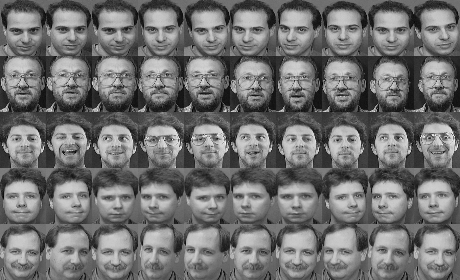
\includegraphics[scale=0.5]{imgs/olivetti_sample.png}
  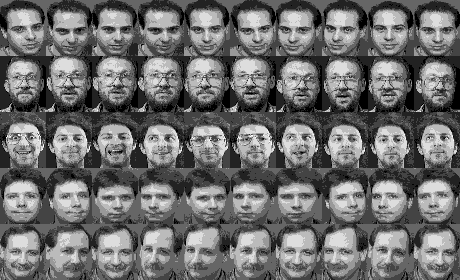
\includegraphics[scale=0.5]{imgs/olivetti-8_sample.png}
  \captionsetup{justification=raggedright}
  \caption{Uma amostra do conjunto de dados Olivetti. A imagem do lado esquerdo é uma amostra do
  \textit{dataset} antes da diminuição de resolução. A imagem do lado direito mostra as imagens com
  resolução de 3-bits.}
\end{figure}

O último conjunto de dados é um \textit{dataset} próprio. Foram criadas 700 imagens de dígitos de 0
a 9, com cada dígito tendo 70 amostras. A variância das imagens em cada categoria é baixa pois o
\textit{dataset} tem como amostra apenas a caligrafia de uma pessoa.

\begin{figure}[h]
  \centering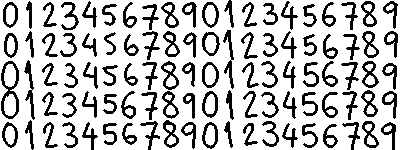
\includegraphics[scale=0.8]{imgs/digits_sample.png}
  \caption{Uma amostra do conjunto de dados Digits.}
\end{figure}

Foram utilizados Caltech-101 e Digits para testes de classificação, e Olivetti para compleição de
imagens. Para cada iteração, foi usado uma porcentagem $p$ para validação cruzada, onde $p$ é a
porcentagem do \textit{dataset} usado para treino, e $1-p$ para teste.

\begin{figure}[h]
  \centering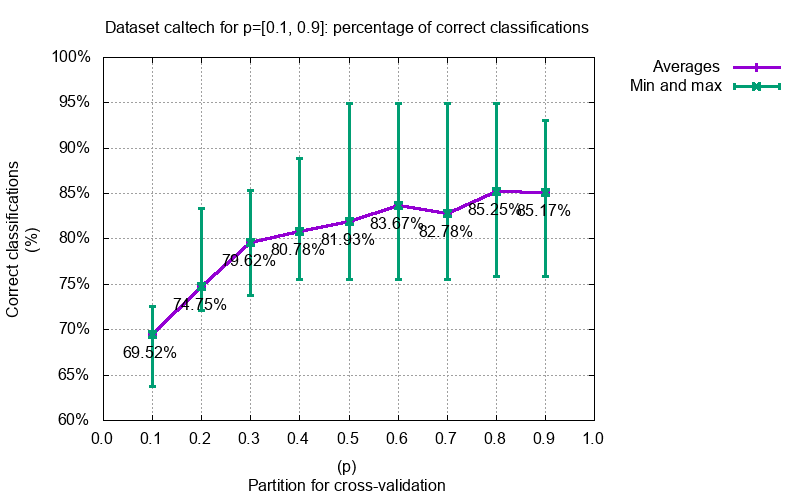
\includegraphics[scale=0.75]{imgs/caltech_percs.png}
  \captionsetup{justification=raggedright}
  \caption{O gráfico mostra a porcentagem de acerto no conjunto de dados Caltech-101 normalizado
  para uma porcentagem $p$ de instâncias usadas para treino. A barra verde mostra as porcentagens
  de acerto máximas e mínimas, enquanto que a linha azul mostra as médias das porcentagens de
  acerto.}
\end{figure}

\begin{figure}[H]
  \centering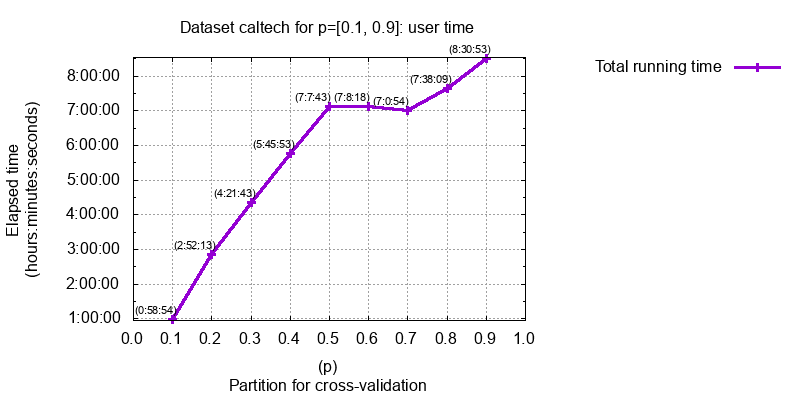
\includegraphics[scale=0.75]{imgs/caltech_time.png}
  \captionsetup{justification=raggedright}
  \caption{O gráfico acima mostra o tempo de aprendizado para cada $p$ no \textit{dataset}
  Caltech-101. O tempo de inferência foi muito menor, na escala de segundos.}
\end{figure}

\begin{figure}[h]
  \centering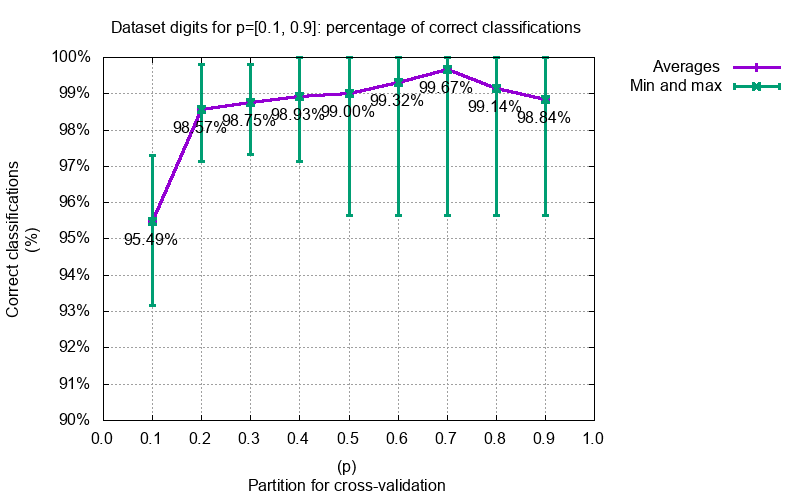
\includegraphics[scale=0.8]{imgs/digits_percs.png}
  \caption{O gráfico mostra a porcentagem de acerto no conjunto de dados Digits.}
\end{figure}

\begin{figure}[H]
  \centering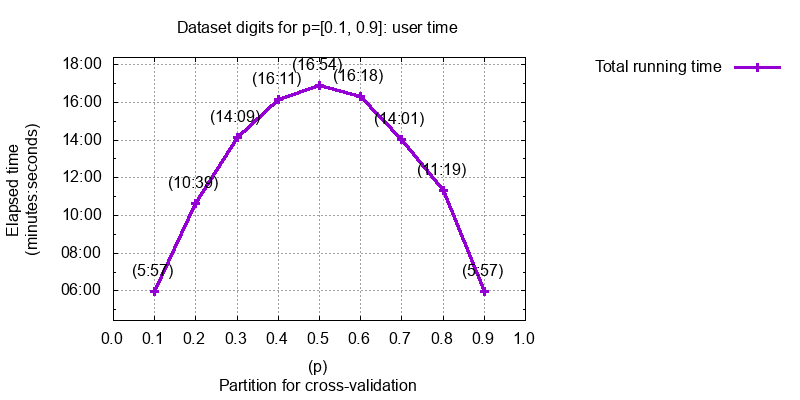
\includegraphics[scale=0.9]{imgs/digits_time.png}
  \caption{O gráfico mostra o tempo de aprendizado para cada $p$ em Digits.}
\end{figure}

O conjunto Olivetti possue 10 imagens de cada pessoa em diferentes ângulos. As imagens
diferenciam-se pela presença de acessórios, como óculos, ou por suas feições faciais, como boca
aberta, sorriso ou olhos fechados.

Para compleição de imagens no conjunto de dados Olivetti, foram aplicados dois testes. Em ambos
testes foi selecionada uma imagem a ser completada, que é então removida do conjunto de treino. No
primeiro teste, o modelo utilizou tanto as imagens de outras pessoas como as 9 imagens restantes da
pessoa a ser completada como conjunto de treino. Chamou-se este método de teste com conhecimento
prévio. Chamou-se de teste sem conhecimento prévio quando apenas utilizamos as faces de outras
pessoas, descartando as 9 restantes.

\begin{figure}[h]
  \centering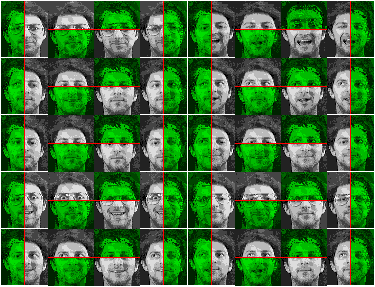
\includegraphics[scale=0.9]{imgs/c1_face_cmpl_39.png}
  \captionsetup{justification=raggedright}
  \caption{O resultado da compleição da parte esquerda da face dada a parte direita do rosto. Neste
  teste houve conhecimento prévio. O modelo percebe a presença de óculos e pêlo facial.}
\end{figure}
\newpage

\begin{figure}[H]
  \centering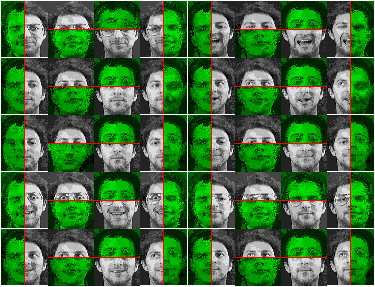
\includegraphics[scale=0.9]{imgs/c2_face_cmpl_39.png}
  \captionsetup{justification=raggedright}
  \caption{A mesma face, porém sem conhecimento prévio. O modelo já não percebe a presença de
  óculos com a mesma taxa de acerto.}
\end{figure}
\newpage

\section{Conclusão}

O objetivo do projeto é o desenvolvimento de uma biblioteca livre e gratuita para inferência e
aprendizado estado-da-arte de redes soma-produto, além de elaborar análises experimentais dos
algoritmos de aprendizado em tarefas de compleição e classificação de imagens. Neste relatório
parcial, foram descritas as atividades desenvolvidas, problemas encontrados e os resultados
parciais realizados durante o período de 01/08/2017 e 31/01/2018. Entre as atividades
desenvolvidas, foram mencionadas funções de inferência, verificação de completude e
decomponibilidade, algoritmos de aprendizado de Gens-Domingos e Poon-Domingos, e geração de
estrutura densa. Por último, foram apresentados resultados parciais em classificação e compleição
de imagem para o algoritmo de Gens-Domingos.

\printbibliography[]

\end{document}
